\usetikzlibrary{calc}
\begin{frame}{baggy bounds check: added code}
    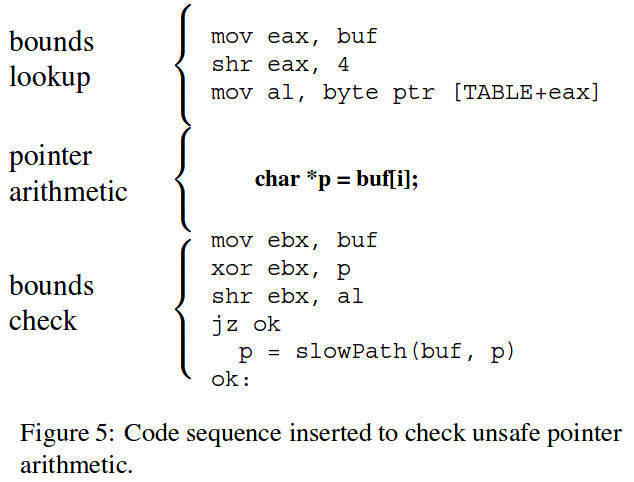
\includegraphics[width=0.6\textwidth]{../bounds/bb-bounds-check}
\end{frame}

\begin{frame}[fragile,label=addedCode]{baggy bounds check: added code}
    \lstset{language=myasm,style=small}
    \begin{lstlisting}
/* bounds lookup */
    mov buf, %rax
    shr %rax, 4
    mov LOOKUP_TABLE(%rax), %al
/* array element address computation */
    ...    // `\textbf{\textit{char * p = buf[i];}}`
/* bound check */
    mov buf, %rbx
    xor p, %rbx
    shr %al, %rbx
    jz  ok
    ...    // handle possible violation
ok:
\end{lstlisting}

    \imagecredit{adapted from paper figure}
\end{frame}

\begin{frame}{avoiding checks}
    \begin{itemize}
        \item code not added if not array/pointer accesses to object
        \item code not added when pointer accesses ``obviously'' safe
            \begin{itemize}
            \item author's implementation: only checked within function
            \end{itemize}
    \end{itemize}
\end{frame}

